\section{Spezifikation der Anforderungen}
Im nun folgenden Unterkapitel werden die im letzten Kapitel, durch Onlinebefragung und in persönlichen Gesprächen, ermittelten Anforderungen spezifiziert, das heißt, systematisch ausgewertet. Es wird aufgrund einer nichtvorhandenen Ausschreibung des Projekts und des geringen Projektumfangs auf ein seperates Lasten- und Pflichtenheft verzichtet und stattdessen die Anforderungen in der hier beginnenden \glqq{}Requirements Specification\grqq{}, zu deutsch \glqq{}Anforderungsspezifikation\grqq{}, niedergeschrieben. Dazu wird sich an der von Helmut Balzert beschriebenen \glqq{}Schablone[n] für Lastenheft, Pflichtenheft und Glossar\grqq{}\footcite[S. 492]{balzert} orientiert. In dieser werden zuerst die Visionen und Ziele des Entwicklungsprojekt verfasst, danach die Rahmenbedingungen denen die Entwicklung unterliegt, im Anschluss der technische Kontext, in dem sich die Entwicklung abspielt und dann erst die funktionalen Anforderungen, die die Kernfunktionalität des Systems beschreiben gefolgt von den nichtfunktionalen Anforderungen, bzw. den Qualitätsanforderungen, in denen die messbare Qualität und das Verhalten des Systems beschrieben wird.\footcite[Vgl.][S. 492 ff.]{balzert}. Die Anforderungen sind natursprachlich verfasst und verfügen über einen einzigartigen Identifikator, um im späteren Verlauf auf sie verweisen zu können. Diese sind so aufgebaut, dass \glqq{} [j]ede Anforderung [..] mit einem Buchstaben [beginnt] [...], gefolgt von einer Zahl, eingschlossen in Schrägstriche. Der Anforderungstyp wird durch einen Buchstaben gekennzeichnet [...].\grqq{} \footcite[S. 493]{balzert}

\subsection{Visionen und Ziele}
Die hier aufgezählten Visionen und Ziele sind Ausdruck der mit dem fertigen Produkt zu erreichenden Zukunft. Visionen sind dabei abstrakter und generisch verfasst, Ziele konkretisieren diese dann im Anschluss.\footcite[Vgl.][S. 457]{balzert}
\begin{itemize}
    \item[] \emph{/V10/} Der Auftraggeber soll durch den Business Transformation Tracker eine Qualitätssteigerung und Effizienzverbesserung in seinen Transformationsprojekten erreichen.
    \item[] \emph{/V20/} Die Anwender sollen mit dem Business Transformation Tracker während des gesamten Projektzeitraums die in SAP umgesetzten Prozesse erfassen und nachverfolgen können.
    \item[] \emph{/V30/} In jedem adesso active transformation -Projekt soll der Business Transformation Tracker eingesetzt werden.
    \item[] \emph{/V40/} Das Produkt soll dem Anwender eine angenehme User Experience bieten und muss ihn in seiner Arbeit produktiv unterstützen.\\
\end{itemize}

\begin{itemize} 
    \item[] \emph{/Z10/} Der Business Transformation Tracker soll zu jedem Zeitpunkt den aktuellen Fortschritssgrad ausgeben können, um schnell eine Übersicht zu erhalten.
    \item[] \emph{/Z20/} Dem Anwender soll es möglich sein, unterschiedliche Projekt aufrufen zu können.
    \item[] \emph{/Z30/} Die Ziele der Informationssicherheit (Authentizität, Vertraulichkeit, Integrität) dürfen nicht verletzt werden.
    \item[] \emph{/Z40/} Alle bereits jetzt implementierten Funktionen werden in die Neuentwicklung übernommen.         
    \item[] \emph{/Z50/} Der Business Transformationen Tracker soll den Funktionsumfang der jetzigen Lösung überbieten.  
    \item[] \emph{/Z60/} Das Anlegen eines Projektes im BTT dauert nicht länger als eine Minute.
    \item[] \emph{/Z70/} Die Erstellung eines Prozesschrittes ist dem Benutzer intuitiv möglich.
    \item[] \emph{/Z80/} Die Anwendung ist auf den verbreitetsten Systemen, Windows, Mac und Linux, einsetzbar.
\end{itemize}

\subsection{Rahmenbedingungen}
Als Rahmenbedingungen bezeichnet man Einschränkungen, die in der Entwicklung der Software berücksichtigt werden müssen. Diese sind entweder technischer oder organisatorischer Natur.\footcite[Vgl.][S. 459 f.]{balzert}
\begin{itemize}
    \item[] \emph{/R10/ Anwendungsbereich:} Das Produkt dient der Transformationsdokumentation in S/4HANA-Transformationsprojekten.
    \item[] \emph{/R20/ Zielgruppen:} Die Projektleiter und -mitarbeiter von adesso orange, die in S/4HANA-Transformationsprojekten eingesetzt werden, sowie die Kunden von adesso orange, die S/4HANA-Projekte in Auftrag geben.
    \item[] \emph{/R30/ Betriebsbedingung:} Büroumgebung und mobiler Einsatz
    \item[] \emph{/R40/ Technische Produktumgebung:} 
    \begin{itemize}
        \item [] \emph{/R41/ Software:} Server-Software: Linux mit Webserver und MySQL Datenbank; Client: x86-Betriebssystem, Google Android oder Apple iOS mit zeitgemäßem Webbrowser.
        \item [] \emph{/R42/ Hardware}: Server: Computer mit 64 Bit x86-Prozessor und zeitgemäßer Ausstattung an Arbeitsspeicher und SSD-Speicher; Client: Mordernes, mobiles Endgerät oder Computer mit 64 Bit x86-Prozessor.
        \item [] \emph{/R43/ Orgware:} Permanenter Internetzugriff und Zugriff auf das adesso VPN.
    \end{itemize}
    \item[] \emph{/R50/ Anforderungen an die Entwicklungsumgebung:} Selbe wie technische Produktumgebung.
\end{itemize}

\subsection{Kontext und Überblick}
Der Kontext beschreibt die technische Umgebebung, in die die Entwicklung eingebettet ist und welche Abhängigkeiten und Schnittstellen zu anderen Systemen exisitieren.\footcite[Vgl.][S. 461 f.]{balzert} Aus den Anforderungen des Systems haben sich keine Schnittstellen zu anderen System ergeben. 

\subsection{Funktionale Anforderungen}
Die Funktionalen Anforderungen beschreiben den Funktionsumfang des Systems. Sie werden im folgenden auf oberster Abstraktionsebene beschrieben und durch Anwendungsfälle (Use-Cases) zusammengefasst, die wiederrum mit der Hilfe von Anwendungsfalldiagrammen dargestellt werden.\footcite[Vgl.][S. 496]{balzert}

\subsubsection{Rollen und Berechtigungen}
\label{kap:RuB}
Zuvor werden jedoch die Akteure der Anwendungsfälle definiert, die sich aus der Anforderungsermittlung und der Stakeholderanalyse ergeben haben. Diese Akteure interagieren mit dem System und sollen später als Benutzerrolle umgesetzt werden. Dazu werden sie hier in einem Rollen- und Berechtigungskonzept beschrieben, damit sie eindeutig spezifiziert sind.

\begin{itemize}
    \item[] \underline{Administrator:} Die Rolle des Administrator ist für die Verwaltung des Systems zuständig, indem er Benutzer anlegt, ihnen Rollen zuweist und Projekte erstellt. Er kann außerdem alle Projekte und darin enthaltenen Teilprojekte einsehen und Änderungen vornehmen. Verkörpert werden die Administratoren durch die Mitarbeiter des oberen Managements des auftraggebenen Unternehmen.
    
    \item[] \underline{Projektleiter:} Die Rolle des Projektleiter ist für die Erstellung und Administration seiner Projekte im System veranwortlich. Im Gegensatz zum Administrator hat der Projektleiter keine vollständigen, globalen Berechtigungen sondern diese nur in seinem eigenen Projekt und kann dort z.B. Teilprojekte anlegen, Projektphasen definieren und Mitarbeiter zuordnen. Zum Ende einer Projektphase kann der Projektleiter die Phase für die Bearbeitung sperren. Auf fremde Projekte hat der Projektleiter keinen Zugriff. 
    
    \item[] \underline{Teilprojektleiter:} Die Rolle des Teilprojektleiter ist für die Verwaltung des ihm zugeordneten Teilprojekts zuständig. In diesem kann er sämtliche Aktionen durchführen, wie z.B. das Bearbeiten von Projektphasenkriterien, das Anlegen von Prozessen, Subprozessen und Prozessschritten und das Erfassen des aktuellen Fortschrittes. Des Weiteren haben Teilprojektleiter Lesezugriff auf fremde Teilprojekte im selben Projekt, um beispielweise Informationen zu übergreifenden Prozessen zu erlangen.

    \item[] \underline{Projektmitarbeiter:} Die Rolle des Projektmitarbeiters ist für die Erfassung in den jeweiligen Teilprojekten zuständig. Der Projektmitarbeiter ist einem Teilprojekt zugeordnet und kann dort Prozesse, Subprozesse und Prozessschritte anlegen und den aktuellen Status erfassen, indem die Kriterien der aktuellen Projektphase entsprechend ausgeprägt werden.

    \item[] \underline{Kunde:} Die Rolle des Kunden soll den Kunden, in dessen Kontext das jeweilige Projekt stattfindet, Zugriff auf das System gewähren. Die Kunden erhalten dabei standardmäßig jeweils nur Lesezugriff auf ihr eigenes Projekt, damit die Fortschritte im Projekt nachvollzogen werden können. Es besteht die Möglichkeit den Benutzern Schreibrechte zu erteilen, entweder für das ganze Projekt, oder nur für einzelne Teilprojekte, um den Fall zu ermöglichen, das Mitarbeiter des Kunden ebenfalls mit dem BTT arbeiten.  
\end{itemize}

\subsubsection{Anwendungsfallübersicht}
Für die Beschreibung der Anwendungsfälle wird auf eine Anwendungsfallschablone zurückgegriffen, die die Eigenschaften des einzelnen Anwendungsfall systematisch abfragt. Die Eigenschaften sind das Ziel des Anwendungsfall, die Kategorie die angibt wie häufig der Anwendungsfall ausgeführt wird, die Vorbedingung, die Nachbedingung bei Erfolg, die Nachbedingung bei Misserfolg, die Akteure des Anwendungsfalls, das auslösende Ereignis, die Beschreibung der einzelnen Schritte, die Erweiterung und mögliche Alternativen.\footcite[Vgl.][S. 261]{balzert}
\begin{figure}[h]
    \centering
    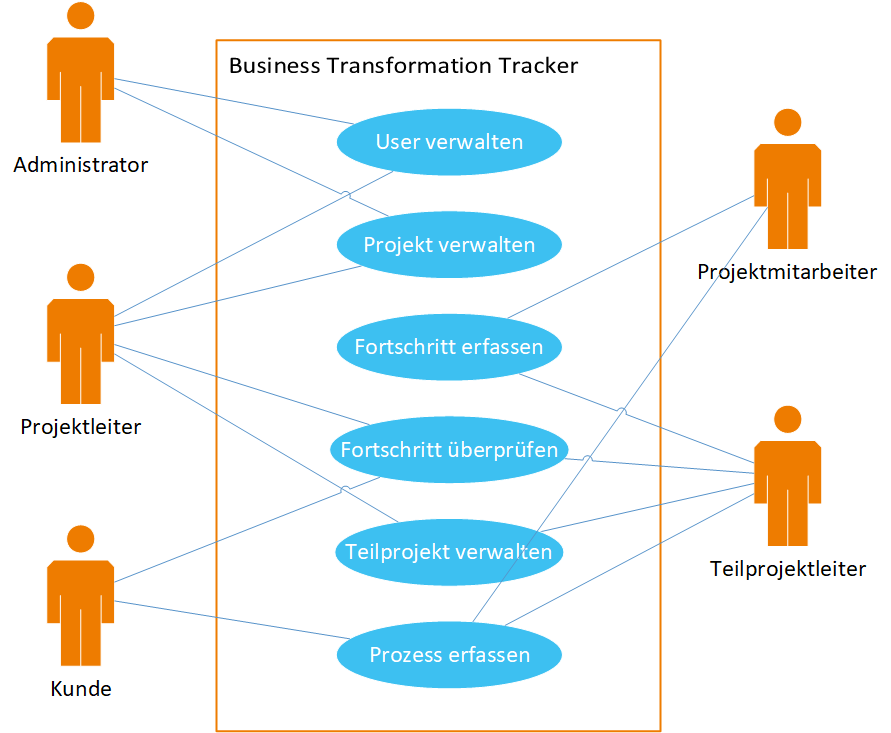
\includegraphics[scale=0.67]{./Bilder/Anwendungsfalldiagramm.png}
    \caption[Anwendungsfalldiagramm]{Anwendungsfalldiagramm mit Akteueren}
    \label{fig:Anwendungsfalldiagramm}
\end{figure}
\\In Abbildung \ref{fig:Anwendungsfalldiagramm} ist eine Übersicht erarbeiteten Anwendungsfälle zu sehen, die in den nachfolgenden Unterkapiteln anhand der oben beschriebenen Schablone genauer spezifiziert werden.

\newpage
\subsubsection{Anwendungsfall 1: Benutzer verwalten}
In der unten dargestellten Tabelle ist der Anwendungsfall \glqq{}Benutzer verwalten\grqq{} beschrieben, der zum Ziel hat die im System hinterlegten Stammdaten der Benutzer zu bearbeiten, die Zuordnung zu einem Projekt oder Teilprojekt durchzuführen, oder die Benutzerrolle zu ändern. Es handelt sich dabei um einen administrativen Anwendungsfall der entweder durch einen Administrator oder einen Projektleiter durchgeführt wird.\\

\begin{tabularx}{\textwidth}{|p{0.33\textwidth}|p{0.612\textwidth}|}
        \hline
        \underline{Ziel:} & Stammdaten, Rolle oder Projektzuordnung des Benutzer verändern \\\hline
        \underline{Kategorie:} & Sekundär \\\hline
        \underline{Vorbedingung:} & Bearbeiter ist mit Benutzername und Passwort angemeldet \\\hline
        \underline{Nachbedingung Erfolg:} & Stammdaten oder Zuordnung des Benutzers wird angepasst \\\hline
        \underline{Nachbedingung Fehlschlag:} & Stammdaten des Benutzers bleiben unverändert \\\hline
        \underline{Akteure:} & Administrator, Projektleiter \\\hline
        \underline{Auslösendes Ereignis:} & Anpassungsbedarf in Stammdaten oder Zuordnung des Benutzers\\\hline        
        \multirow{1}{*}{\underline{Beschreibung:}} & [1] Auswählen des Benutzers \\
        & [2] Änderung der Stammdaten \\\hline
        \multirow{1}{*}{\underline{Erweiterung:}} & [1a] Benutzer wird angelegt \\
        & [2a] Änderung der Projektzuordnung \\
        & [2b] Änderung der Teilprojektzuordnung \\
        & [2c] Änderung der Benutzerrolle \\\hline
        \underline{Alternativen:} & ./. \\\hline
\end{tabularx}
\captionof{table}[Anwendungsfall 1: Benutzer verwalten ]{Benutzer verwalten}
\newpage
In Abbildung \ref{fig:AD1} sind die Aktivitäten des oben beschriebenen Anwendungsfalls \glqq{}Benutzer verwalten\grqq{} abgebildet, die im System durchgeführt werden um das gewünscht Ziel zu erreichen. Das Aktivitätsdiagramm stellt dabei, die Schritte des Ablaufs visuell dar.
\begin{figure}[h!]
    \centering
    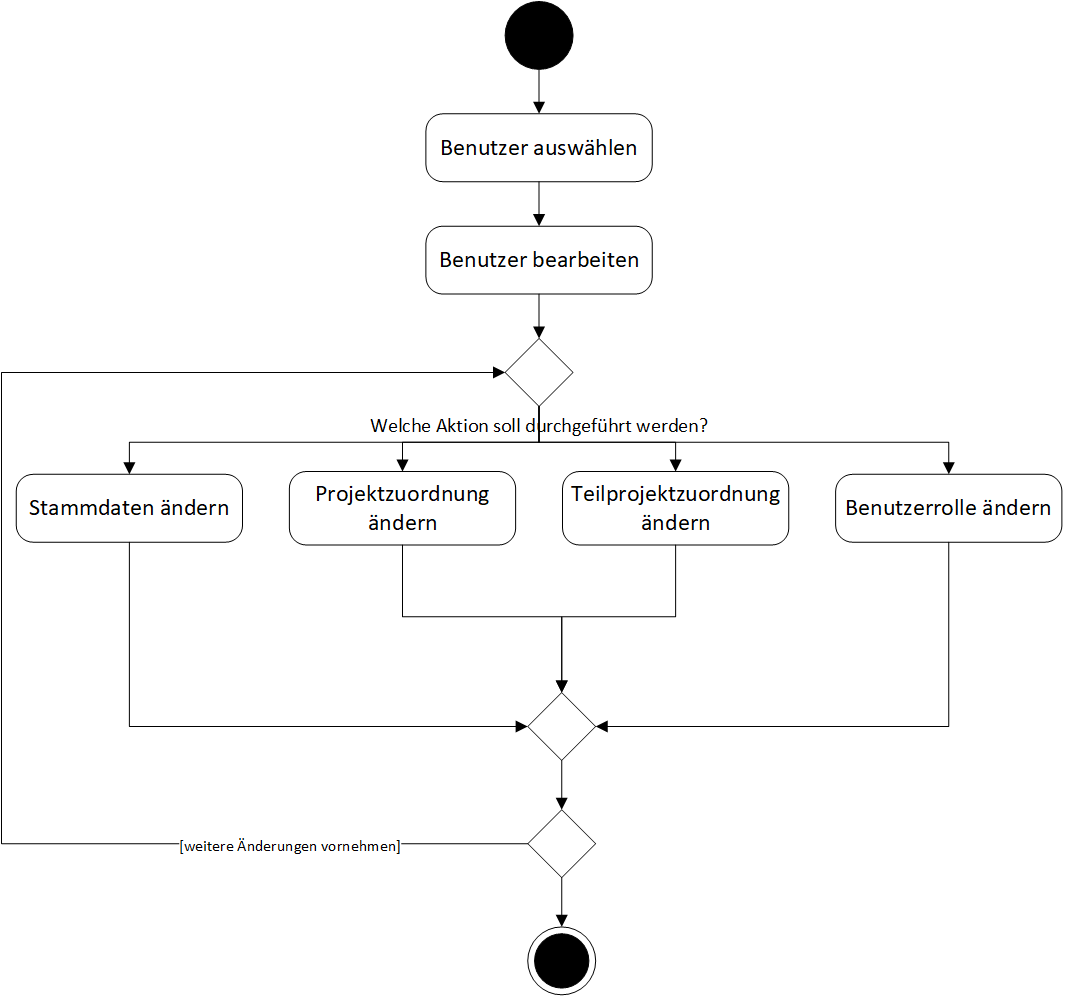
\includegraphics[scale=0.67]{./Bilder/AD1_BenutzerVerwalten.png}
    \caption[Aktivitätsdiagramm Anwendungsfall 1]{Aktivitätsdiagramm Benutzer verwalten}
    \label{fig:AD1}
\end{figure}
\\Mit der Aktivität \glqq{}Benutzerrolle ändern\grqq{} kann der Bearbeiter die Rolle des ausgewählten Nutzers verändern. Die Rollen, die bereits in den vorherigen Kapiteln erwähnt wurden, stellen die jeweilige Position im Projekt dar. Die Aktivität kann durch die Rolle Projektleiter und Administator durchgeführt werden, jedoch kann ein Projektleiter keine Administatorrolle vergeben.

\newpage
\subsubsection{Anwendungsfall 2: Projekt anlegen}
Nachfolgend Tabelle wird der Anwendungsfall \glqq{}Projekt anlegen\grqq{} beschrieben. Dieser zeigt das Vorgehen zum Anlegen eines neues Projektes im System auf. Das Vorgehen wird zuerst in der Anwendungsfallschablone beschrieben und im Anschluss durch ein Aktivitätsdiagramm beschrieben.\\

\begin{tabularx}{\textwidth}{|p{0.33\textwidth}|p{0.612\textwidth}|}
        \hline
        \underline{Ziel:} & Ein neues Projekt wird im System angelegt.\\\hline
        \underline{Kategorie:} & Primär\\\hline
        \underline{Vorbedingung:} & Der Anwender ist mit Benutzername und Passwort angemeldet; Projekt ist noch nicht angelegt.\\\hline
        \underline{Nachbedingung Erfolg:} & Das Projekt wird angelegt; Stammdaten werden hinterlegt; Projektphasen sind vorhanden; Teilprojekte sind vorhanden; Benutzer sind zugeordnet.\\\hline
        \underline{Nachbedingung Fehlschlag:} & System bleibt unverändert.\\\hline
        \underline{Akteure:} & Administrator, Projektleiter\\\hline
        \underline{Auslösendes Ereignis:} & adesso orange beginnt neues S/4HANA-Transformationsprojekt.\\\hline        
        \multirow{1}{*}{\underline{Beschreibung:}} & [1] Projekt hinzufügen\\
        & [2] Stammdaten anlegen\\
        & [3] Teilprojekt anlegen\\
        & [4] Projektphase anlegen\\
        & [5] Mitarbeiter zuordnen\\\hline
        \multirow{1}{*}{\underline{Erweiterung:}} & [3a] Weiteres Teilprojekt anlegen\\
        & [4a] Weitere Projektphase hinzufügen\\\hline
        \underline{Alternativen:} & [4b] Kriterien hinzufügen\\\hline
\end{tabularx}
\captionof{table}[Anwendungsfall 2: Projekt anlegen]{Projekt anlegen}
\newpage
Nachfolgend wird in Abbildung \ref{fig:AD2} das Aktivitätsdiagramm dargestellt. Dies zeigt den Ablauf des Anwendungsfalls 2 detailliert auf und zeigt die Schritte, die der Anwender durchführen muss um im System erfolgreich ein Projekt anzulegen.
\begin{figure}[h!]
    \centering
    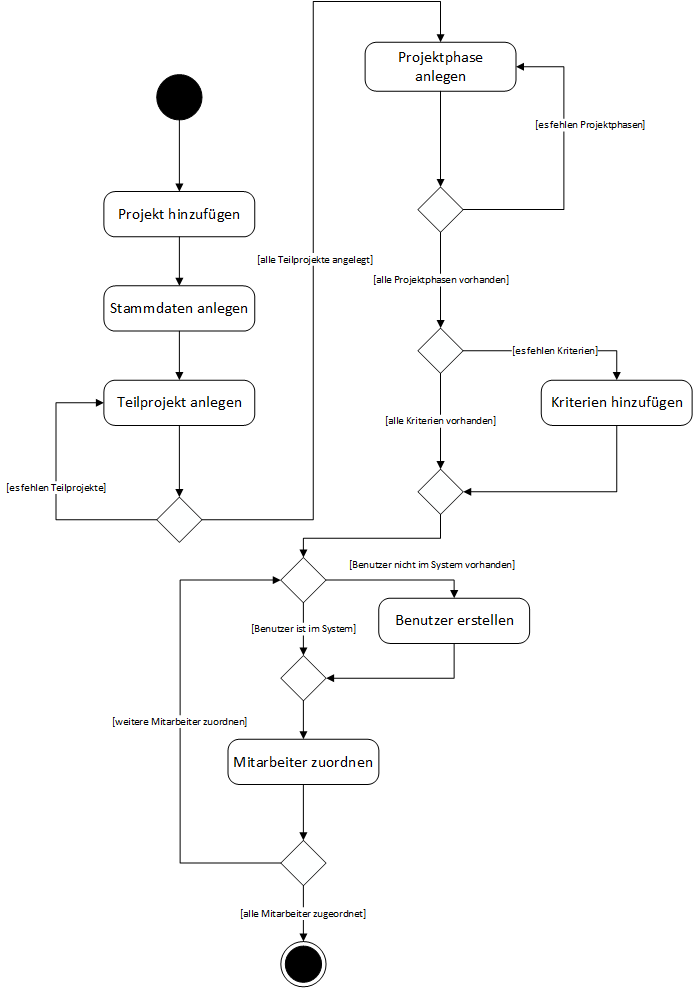
\includegraphics[scale=0.67]{./Bilder/AD2_ProjektAnlegen.png}
    \caption[Aktivitätsdiagramm Anwendungsfall 2]{Aktivitätsdiagramm Projekt anlegen}
    \label{fig:AD2}
\end{figure}
\\Dieses Diagramm wird im ersten Moment sehr komplex, da es viele für den Erstellers des Projektes viele Entscheidungsmöglichkeiten gibt, wie umfangreich das Projekt anlegt wird. 

\newpage
\subsubsection{Anwendungsfall 3: Teilprojekt verwalten}
Der Anwendungsfall 3 \glqq{}Teilprojekt verwalten\grqq{} beschreibt die Bearbeitung eines Teilprojekts aus Sicht eines Teilprojektleiters. Dieser kann in dem ihn zugewiesenen Teilprojekt die Stammdaten ändern, die Kriterien der Projektphasen anpassen und Mitarbeiter dem Teilprojekt zuweisen.\\

\begin{tabularx}{\textwidth}{|p{0.33\textwidth}|p{0.612\textwidth}|}
        \hline
        \underline{Ziel:} & Änderung in Teilprojekt durchführen durch Stammdatenänderung, Kriteriennderung oder Mitarbeiterzuweisung \\\hline
        \underline{Kategorie:} & Sekundär\\\hline
        \underline{Vorbedingung:} & Der Anwender ist mit Benutzername und Passwort angemeldet; Projekt mit Teilprojekt(en) und Projektphase(n) ist angelegt; Bearbeiter ist Projekt zugeordnet\\\hline
        \underline{Nachbedingung Erfolg:} & Daten im Teilprojekt geändert \\\hline
        \underline{Nachbedingung Fehlschlag:} & Keine Änderungen durchgeführt \\\hline
        \underline{Akteure:} & Projektleiter, Teilprojektleiter \\\hline
        \underline{Auslösendes Ereignis:} & Neue Mitarbeiter im Teilprojekt; Stammdaten müssen angepasst werden\\\hline        
        \multirow{1}{*}{\underline{Beschreibung:}} & [1] Aufruf Teilprojekt\\
        & [2] Bearbeitung der Stammdaten\\\hline
        \multirow{1}{*}{\underline{Erweiterung:}} & [2a] Mitarbeiter zuordnen\\
        & [2b] Kriterium ändern\\\hline
        \underline{Alternativen:} & ./. \\\hline
\end{tabularx}
\captionof{table}[Anwendungsfall 3: Teilprojekt verwalten]{Teilprojekt verwalten}
\newpage
Nachfolgend ist in Abbildung \ref{fig:AD3} das Aktivitätsdiagramm für den Anwendungsfall \glqq{}Teilprojekt verwalten\grqq{} dargestellt.
\begin{figure}[h!]
    \centering
    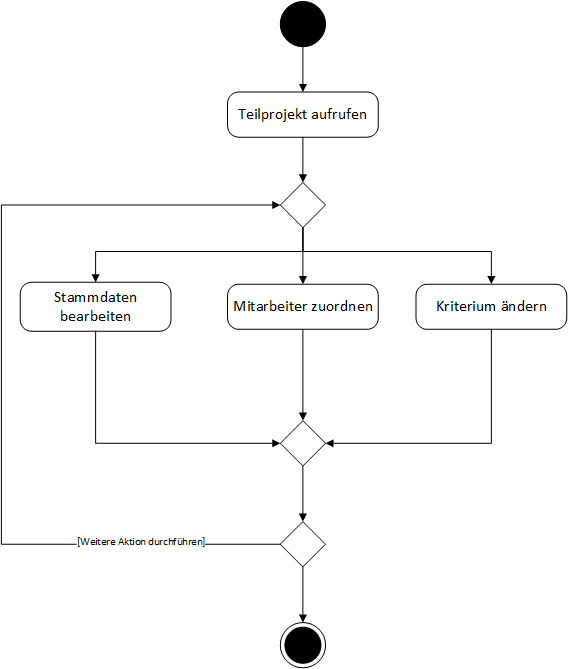
\includegraphics[scale=0.67]{./Bilder/AD3_TeilprojektVerwalten.png}
    \caption[Aktivitätsdiagramm Anwendungsfall 3]{Aktivitätsdiagramm Teilprojekt verwalten}
    \label{fig:AD3}
\end{figure}
\\Im Mittelpunkt dieses Anwendungsfalls steht die Entscheidung, welche Aktion durchgeführt werden soll. Hier kann der Anwender auswählen, ob er die Stammdaten bearbeitet, einen weiteren Mitarbeiter zuordnet oder ein Kriterium anpasst. Im Anschluss an die Durchführung einer Aktivität kann der Anwender erneut entscheiden, ob er eine weitere Aktion durchführen möchte, bis schließlich alle gewünschten Anpassungen durchgeführt wurden.

\newpage
\subsubsection{Anwendungsfall 4: Prozess erfassen}
In der unten abgebildeten Tabelle ist der Anwendungsfall \glqq{}Prozess erfassen\grqq{} beschrieben, der zu beginn eines S/4HANA-Transformationsprojekts zur Anwendung kommt, wenn, in Zusammenarbeit mit den Kunden, die in SAP abgebildeten Prozesse in ihrer Gesamtheit aufgenommen werden.\\

\begin{tabularx}{\textwidth}{|p{0.33\textwidth}|p{0.612\textwidth}|}
        \hline
        \underline{Ziel:} & Kundenprozess inklusive aller Schritte erfassen \\\hline
        \underline{Kategorie:} & Primär\\\hline
        \underline{Vorbedingung:} & Der Anwender ist mit Benutzername und Passwort angemeldet; Projekt mit Teilprojekt(en) und Projektphase(n) ist angelegt; Bearbeiter ist Projekt und Teilprojekt zugeordnet\\\hline
        \underline{Nachbedingung Erfolg:} & Neuer Prozess mit jeweiligen Schritten wird hinterlegt \\\hline
        \underline{Nachbedingung Fehlschlag:} & Kein neuer Prozess im System vorhanden oder Prozess unvollständig erfasst. \\\hline
        \underline{Akteure:} & Teilprojektleiter, Projektmitarbeiter, Kunde\\\hline
        \underline{Auslösendes Ereignis:} & Zu Beginn eines Projekts sollen Prozesse erfasst werden.\\\hline        
        \multirow{1}{*}{\underline{Beschreibung:}} & [1] Projekt aufrufen\\
        & [2] Teilprojekt aufrufen\\
        & [3] Neuen Prozess anlegen\\
        & [4] Stammdaten des Prozess erfassen\\
        & [5] Neuen Prozessschritt anlegen\\
        & [6] Daten des Prozessschritts erfassen.\\\hline
        \multirow{1}{*}{\underline{Erweiterung:}} & [5a] Subprozess anlegen\\
        & [5a] Daten des Subprozess erfassen\\\hline
        \underline{Alternativen:} & ./. \\\hline
\end{tabularx}
\captionof{table}[Anwendungsfall 4: Prozess erfassen]{Prozess erfassen}
\newpage
In Abbildung \ref{fig:AD4} ist die Abfolge der Aktivitäten zur Erfassung eines neuen Prozesses abgebildet. Mit dieser Abfolge ist es möglich Prozesse zu erfassen, die entweder nur in einem Teilprojekt stattfinden, oder die sich über mehrere Teilprojekt erstrecken. 
\begin{figure}[h!]
    \centering
    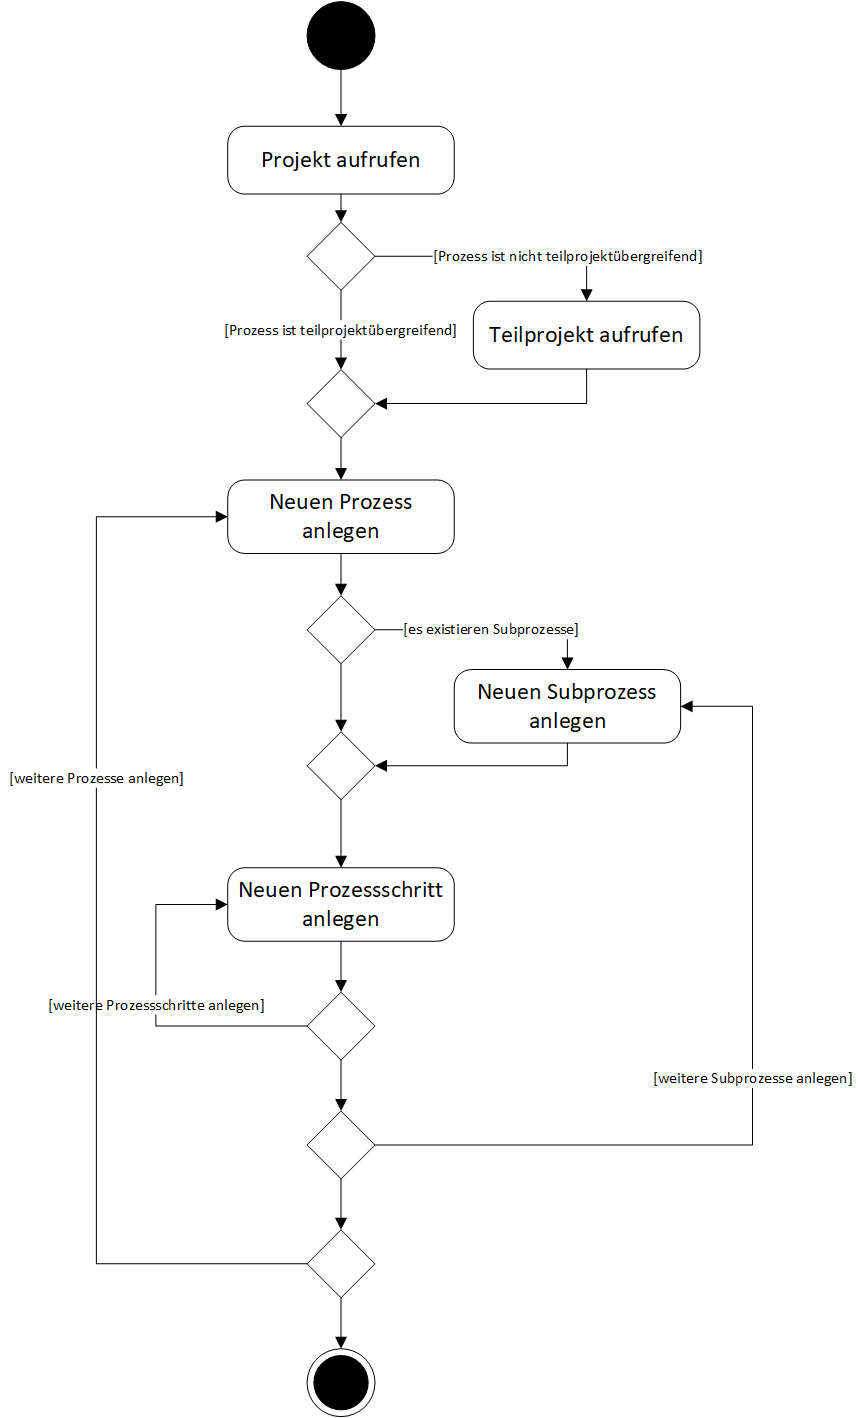
\includegraphics[scale=0.67]{./Bilder/AD4_ProzessErfassen.png}
    \caption[Aktivitätsdiagramm Anwendungsfall 4]{Aktivitätsdiagramm Prozess erfassen}
    \label{fig:AD4}
\end{figure}
\\Danach werden nach und nach alle Einzelheiten des Prozess erfasst, sodass dieser mit all seinen Subprozessen und einzelnen Prozessschritten im System abgebildet wird. Der Anwender hat am Ende der Aktivitätenabfolge jedes Mal die Möglichkeit weitere Aktionen durchzuführen, indem er an den Anfang des Prozess zurückkehrt.

\newpage
\subsubsection{Anwendungsfall 5: Fortschritt erfassen}
Der Anwendungsfall \glqq{}Fortschritt erfassen\grqq{} dient dazu den in der S/4HANA-Transformation geleisteten Fortschritt, bzw. die Abarbeitung einer geleisteten Transformationsaufgabe, im System zu erfassen und ihn dadurch zu dokumentieren.\\

\begin{tabularx}{\textwidth}{|p{0.33\textwidth}|p{0.612\textwidth}|}
        \hline
        \underline{Ziel:} & Im Projekt geleisteten Fortschritt dokumentieren \\\hline
        \underline{Kategorie:} & Primär \\\hline
        \underline{Vorbedingung:} & Der Benutzer ist mit Benutzername und Passwort angemeldet; Projekt mit Teilprojekt(en) und Projektphase(n) ist angelegt; Bearbeiter ist Projekt und Teilprojekt zugeordnet \\\hline
        \underline{Nachbedingung Erfolg:} & Projektphasenkriterien werden ausgefüllt; Fortschrittsanzeige verändert sich \\\hline
        \underline{Nachbedingung Fehlschlag:} & Keine Änderung in Projektphasenkriterien; Fortschrittsanzeige bleibt gleich \\\hline
        \underline{Akteure:} & Teilprojektleiter; Projektmitarbeiter \\\hline
        \underline{Auslösendes Ereignis:} & Im Transformationsprozess wurde Aufgabe abgearbeitet (Außerhalb des IT-Systems)\\\hline        
        \multirow{1}{*}{\underline{Beschreibung:}} & [1] Projekt aufrufen \\
        & [2] Teilprojekt aufrufen \\
        & [3] Prozess aufrufen \\
        & [4] Projektphasenkriterium mit Wert befüllen \\\hline
        \multirow{1}{*}{\underline{Erweiterung:}} & [4a] Weitere Projektphasenkriterien verändern \\\hline
        \underline{Alternativen:} & ./. \\\hline
\end{tabularx}
\captionof{table}[Anwendungsfall 5: Fortschritt erfassen]{Fortschritt erfassen}
\newpage
In dem in Abbildung \ref{fig:AD5} dargestellten Aktivitätsdiagramm sind die Schritte zur Fortschrittserfassung im System abgebildet.
\begin{figure}[h!]
    \centering
    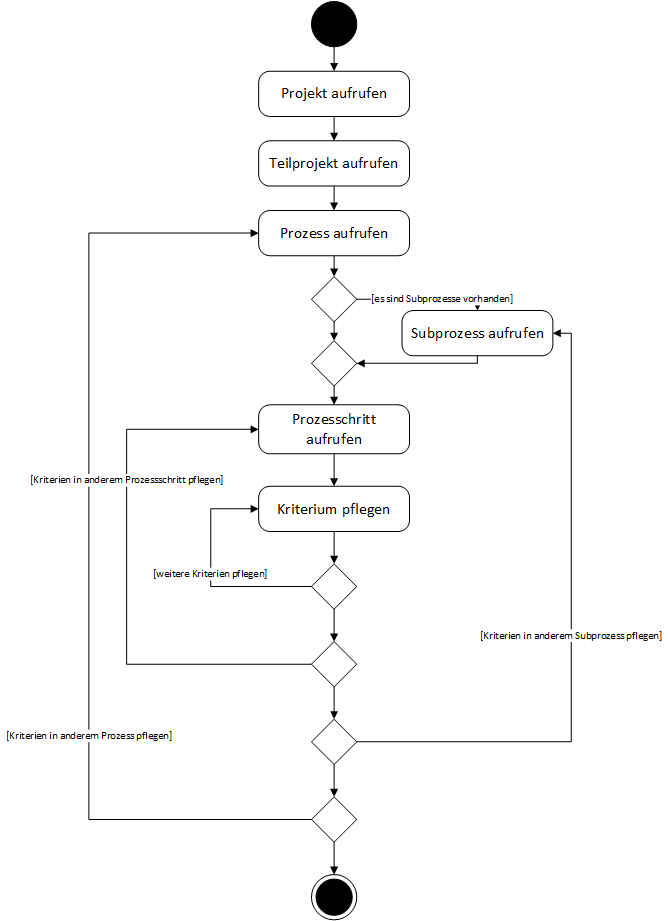
\includegraphics[scale=0.67]{./Bilder/AD5_FortschrittErfassen.png}
    \caption[Aktivitätsdiagramm Anwendungsfall 5]{Aktivitätsdiagramm Fortschritt erfassen}
    \label{fig:AD5}
\end{figure}
\\Diese Erfassung wird durch die Ausprägung der Projektphasenkriterien im System vorgenommen. Dazu wird zuerst der Prozess und im nachfolgenden Verlauf ein einzelner Prozessschritt aufgerufen und dort die Ausprägung der Kriterien gepflegt.
\newpage
\subsubsection{Anwendungsfall 6: Fortschritt überprüfen}
Der Anwendungsfall 6 \glqq{}Fortschritt überprüfen\grqq{} beschreibt das Vorgehen zur Überprüfung des geleisteten Fortschrittes. Dies geschieht durch ein eigens dafür vorgesehenes Dashboard, das auf einem Blick den Fortschritt eines Projektes wiederspiegelt.\\
\begin{tabularx}{\textwidth}{|p{0.33\textwidth}|p{0.612\textwidth}|}
        \hline
        \underline{Ziel:} & Aktuellen Fortschritt einer Projektphase wiedergeben\\\hline
        \underline{Kategorie:} & Sekundär \\\hline
        \underline{Vorbedingung:} & Der Benutzer ist mit Benutzername und Passwort angemeldet; Projekt mit Teilprojekt(en) und Projektphase(n) ist angelegt; Bearbeiter ist Projekt und Teilprojekt zugeordnet\\\hline
        \underline{Nachbedingung Erfolg:} & Es wird die gewünschte Auswertung ausgegeben\\\hline
        \underline{Nachbedingung Fehlschlag:} &  Es wird keine Auswertung wiedergegeben, diese muss bei durch Befragung der Mitarbeiter manuell erhoben werden.\\\hline
        \underline{Akteure:} & Projektleiter, Teilprojektleiter, Kunde \\\hline
        \underline{Auslösendes Ereignis:} & Regelmäßige Erhebung des Fortschrittes bspw. im Rahmen eines Jour Fixes \\\hline        
        \multirow{1}{*}{\underline{Beschreibung:}} & [1] Projekt aufrufen\\
        & [2] Projektdashboard aufrufen\\\hline
        \multirow{1}{*}{\underline{Erweiterung:}} & ./. \\\hline
        \underline{Alternativen:} & [3a] Teilprojekt aufrufen (detaillierte Auswertung)\\\hline
\end{tabularx}
\captionof{table}[Anwendungsfall 6: Fortschritt überprüfen]{Fortschritt überprüfen}
\newpage
In Abbildung \ref{fig:AD6} sind die Aktivitäten visualisiert, die durchgeführt werden müssen, um eine Auswertung zu erhalten.
\begin{figure}[h!]
    \centering
    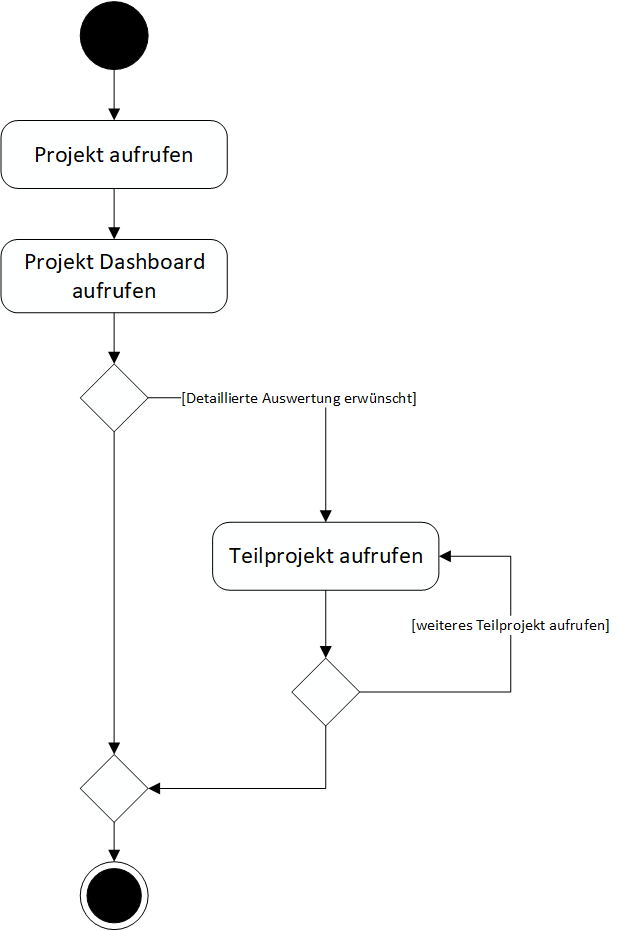
\includegraphics[scale=0.67]{./Bilder/AD6_FortschrittÜberprüfen.png}
    \caption[Aktivitätsdiagramm Anwendungsfall 6]{Aktivitätsdiagramm Fortschritt überprüfen}
    \label{fig:AD6}
\end{figure}
\\Dies geschieht entweder über das Dashboard, das eine Übersicht über und das Projekt und seine Teilprojekte liefert, oder über den Aufruf der einzelnen Teilprojekte, in denen der Fortschritt detaillierter Beguachtet werden kann.
\newpage
\subsection{Qualitätsanforderungen}
Die nichtfunktionalen Anforderungen, bzw. Qualitätsanforderungen spiegeln Eigenschaften wieder, die das gesamte System und somit alle funktionalen Anforderungen betreffen. Die Qualitätsanforderungen werden anhand unterschiedlicher Kriterien kategorisiert, der \textbf{F}unktionalität, der \textbf{Z}uverlässigkeit, der \textbf{B}enutzbarkeit, der \textbf{E}ffizienz, der \textbf{W}artbarkeit und der \textbf{P}ortabilität.\footcite[Vgl.][S. 494 f.]{balzert} Die ermittelten nichtfunktionalen Anforderungen lauten wie folgt:
\vspace{0.5cm}
\\\textbf{Funktionalität:}
\begin{itemize}
    \item[] \emph{/QF10/} Das System darf nur über eine gesicherte Verbindung mit SSL-Ver-schlüsselung erreichbar sein.
    \item[] \emph{/QF20/} Die Anwender dürfen nur die Aktionen der ihr zugeordneten Rolle (siehe Kapitel \ref{kap:RuB}) ausführen dürfen.
    \item[] \emph{/QF30/} Alle Benutzer verfügen über personalisierte Benutzernamen und Passwörter.
    \item[] \emph{/QF31/} Die Passwörter der Benutzerkonten müssen den \glqq{}Digital Identity Guidlines\grqq{} des NIST (National Institute of Standards and Technology) entsprechen\footnote{Siehe: https://doi.org/10.6028/NIST.SP.800-63b}
    \item[] \emph{/QF40/} Die Eingabefelder des Systems müssen gegen SQL-Injecting und Cross-Site-Scripting gesichert sein.
\end{itemize}
\vspace{0.5cm}
\textbf{Zuverlässigkeit:}
\begin{itemize}
    \item[] \emph{/QZ10/} Das System soll eine Verfügbarkeit von 98 Prozent im Jahr haben.
    \item[] \emph{/QZ20/} Es werden regelmäßige Sicherungen der Daten durchgeführt.
    \item[] \emph{/QZ30/} Fehler in der Anwendung führen nur zum Absturz, wenn dieses unvermeidbar ist.
\end{itemize}
\vspace{0.5cm}
\textbf{Benutzbarkeit:}
\begin{itemize}
    \item[] \emph{/QB10/} Das System verfügt über eine grafische Benutzeroberfläche.
    \item[] \emph{/QB20/} Es gibt eine Anwenderdokumentation.
\end{itemize}
\vspace{0.5cm}
\textbf{Effizienz:}
\begin{itemize}
    \item[] \emph{/QE10/} Die Reaktionszeiten des Systems betragen bei einer stabilen Internetverbindung weniger als 5 Sekunden.
    \item[] \emph{/QE20/} Speichervorgänge dürfen nicht länger als 5 Sekunden dauern.  
\end{itemize} 
\vspace{0.5cm}
\textbf{Wartbarkeit:}
\begin{itemize}
    \item[] \emph{/QW10/} Es finden regelmäßige Updates der Serversoftware statt.
    \item[] \emph{/QW20/} Das System speichert Protokolle über von dem Benutzer ausgeführte Aktionen. (TBD) 
    \item[] 
\end{itemize}
\vspace{0.5cm}
\textbf{Portabilität:}
\begin{itemize}
    \item[] \emph{/QP10/} Der kleinste unterstützte Bildschirm hat eine Bilddiagonale von 4,7 Zoll mit einer Auflösung von 1334 x 750 Pixeln (iPhone 6).
    \item[] \emph{/QP20/} Die Benutzeroberfläche der Anwendung ist durch den Benutzer frei in ihrer Größe skalierbar.
\end{itemize}

\begin{comment}
    Use cases
    1. Tägliches Statusupdates zur Besprechung des Fortschrittes in den Teilprojekten
    2. Anlegen eines Projektes mit seinen jeweiligen Teilprojekten und Projektphasen, Zuordnung der Rollen
    3. Initiales Erfassen eines Prozesses, mit seinen Subprozessen und den Prozessschritten
    4. Pflegen der Felder einer Projektphase 
    5. Abschließen einer Projektphase.

    Akteuere im System
    - Eigentümer des Projekts, Admin, oberes Mgmnt.
    - Projektleiter (n, normalfall 2)
    - Projektcontroller (read only)
    - Teilprojektleiter
    - Projektmitarbeiter

    \begin{itemize}
        \item[] \emph{/F10/} Die Anwendung benutzt eine grafische Oberfläche.
        
        \item[] \emph{/F20/} Es gibt unterschiedliche Benutzerrollen im System.
        
        \item[] \emph{/F30/} Die Benutzerrollen haben unterschiedliche Berechtigungen.
        \item[] \emph{/F31/} Der Benutzer loggt sich mit Benutzername und Passwort ein.
        
        \item[] \emph{/F40/} Es können ein oder mehrere Projekte angelegt und aufgerufen werden.
        
        \item[] \emph{/F50/} Ein Projekt besteht aus mehreren Projektphasen.
        \item[] \emph{/F51/} Die Projektphasen werden auf die Teilprojekte vererbt.
        
        \item[] \emph{/F60/} Innerhalb eines Projektes können ein oder mehrere Teilprojekte erstellt werden.
        
        \item[] \emph{/F70/} Innerhalb eines Projektes werden Prozesse aufgenommen
        \item[] \emph{/F80/} Die Prozesse können einem Teilprojekt zugeordnet werden oder nicht.
        \item[] \emph{/F90/} Innerhalb eines Prozesses können keine oder mehere Subprozesse aufgenommen werden.
        \item[] \emph{/F100/} Ein (Sub-)Prozess besteht aus einem oder mehreren Prozessschritten
        \item[] \emph{/F110/} Ein Prozessschritt muss einem Teilprojekt zugeordnet sein.
        \item[] \emph{/F120/}      
    \end{itemize}
    
\end{comment}
    